\documentclass[
  aspectratio=169,
]{beamer}

% Základní definice
\usepackage[greek,czech]{babel}
\usepackage[utf8]{inputenc}
\usepackage[T1]{fontenc}
\usepackage{hologo}
\usetheme[
  workplace=fi,
]{MU}
\bibliographystyle{czechiso}

% Rozšiřující makra
\newcommand\odkaz[2]{\textcolor{mubeamer@base}{\href{#1}{#2}}}
\providecommand\doi{doi:\textcolor{mubeamer@base}}

\begin{document}

\title[\TeX{} na MU]{\TeX{} na Masarykově univerzitě}
\subtitle{Šablony fithesis, mubeamer a~muletter}
\author[V.\,Novotný]{Mgr.\ Vít Novotný \\ witiko@mail.muni.cz}
\institute[FI MU]{Faculty of Informatics, Masaryk University}
\date{10.\ října 2018}
\subject{TeX na Masarykově univerzitě}
\keywords{tex, latex, template}

\begin{frame}[plain]
\maketitle
\end{frame}

\begin{frame}{Obsah}
\tableofcontents
\end{frame}

\section[Stručná historie \TeX u na MU]{Stručná historie \TeX u na Masarykově univerzitě}

\begin{frame}{Stručná historie \TeX u na Masarykově univerzitě}
\begin{itemize}
\item \TeX{} -- řecký kořen slov \alert{technologie} (\textgreek{τεχνολογία}) a~\alert{umění} (\textgreek{τέχνη}) -- je \alert{programovací jazyk} navržený v~70. a~80. letech 20. století na Stanfordské univerzitě \alert{pro knižní sazbu s~důrazem na matematiku}. $\forall a,b\in\mathbb{Z}: a\mid b\iff\exists c\in\mathbb{Z}:a\cdot c=b$
\item V~Československu 80. let sloužil \TeX{} pro šíření informací samizdatovou komunitou.
\item V~90. letech se ÚVT MU stává kolektivním členem sdružení \TeX{} Users Group (TUG).
\item V~roce 1994 je založena FI, \alert{\TeX em sázíme rozvrhy, telefonní seznamy a~diplomy}. \TeX{} se stává \alert{integrální součástí IS MU} a používá se pro výstupy všech fakult.~\cite{sojkanovotny17} Pomocí \TeX u bylo připraveno i~logo nové fakulty~\cite{zlatuska95}, ligatura FI jako symbol kvalitní typografie. 
\item V~roce 1996 vzniká na FI program pdf\TeX{}, který umožňuje generovat PDF výstup. Pdf\TeX{} je dnes \alert{světový de-facto standard pro přípravu matematických publikací}.
\end{itemize}
\end{frame}

\section[\TeX ové šablony MU]{\TeX ové šablony Masarykovy univerzity}
\subsection{Šablona fithesis}

\begin{frame}{Šablona fithesis}
\begin{itemize}
\item V~roce 1998 vznikla na FI \TeX ová \alert{šablona fithesis pro sazbu závěrečných prací}.
\item V~roce 2004 přibyla do šablony fithesis slovenská lokalizace.
\item V~roce 2008 přibyla do druhé verze šablony, \alert{fithesis2, loga ostatních fakult MU}.
\item V~roce 2013 přibyla do šablony fithesis2 podpora fontů Comenia zakoupených~FI.
\item V~roce 2015 přibyla do třetí verze šablony, \alert{fithesis3~\cite{novotny15}, plná podpora směrnic jednotlivých fakult MU}. Zároveň vzniklo v~IS MU \odkaz{https://is.muni.cz/auth/df/fithesis-sazba/}{diskuzní fórum uživatelů \TeX u}.
\item V~roce 2016 přibyla do šablony fithesis3 podpora automatického generování bibliografických odkazů a~citací podle ČSN ISO 690:2013.
\end{itemize}
\end{frame}

\begin{frame}{Počty přístupů k~šabloně fithesis3 podle fakult}
\kern-1.5em\leavevmode\kern-0.05\textwidth\relax
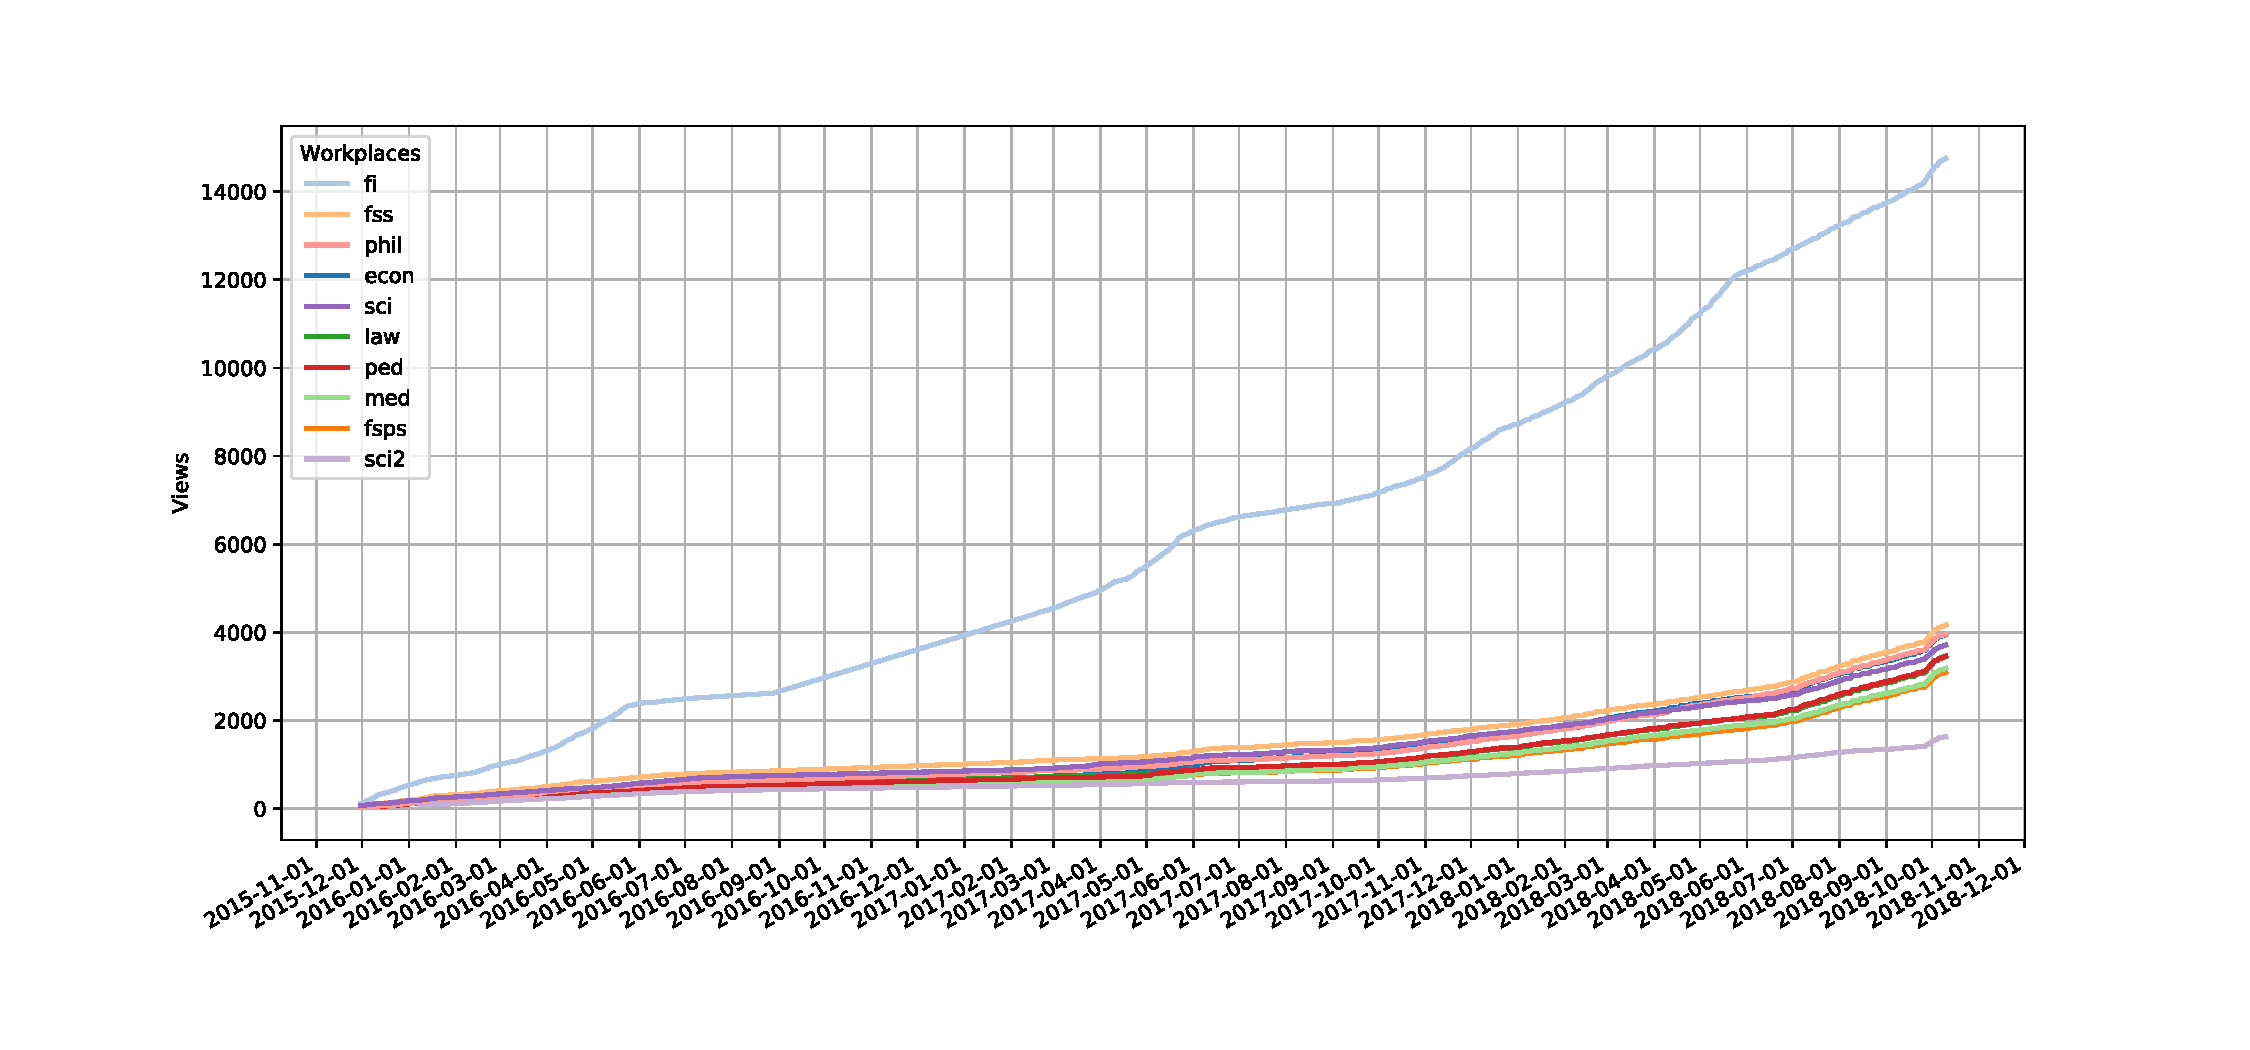
\includegraphics[width=1.1\textwidth]{figs/fithesis}
\end{frame}

\subsection{Šablona mubeamer}

\begin{frame}{Šablona mubeamer}
\begin{itemize}
\item V~roce 2015 vznikla na FI \TeX ová \alert{šablona fibeamer pro sazbu prezentací k~obhajobám závěrečných prací na všech fakultách MU}.
\item V~roce 2016 přibyla do šablony fibeamer částečná podpora JVS MU 2016.
\item V~roce 2017 vznikla ve spolupráci ÚVT MU a~FI \alert{šablona mubeamer pro sazbu prezentací podle JVS MU 2016 na 28 pracovištích MU}.
\end{itemize}

\begin{block}{Příklad}
Pracoviště, pro které je prezentace určena, lze snadno změnit bez zásahu do samotného obsahu dokumentu.
\end{block}
\end{frame}

\begin{frame}{Počty přístupů k~šabloně fibeamer podle fakult}
\kern-1.5em\leavevmode\kern-0.05\textwidth\relax
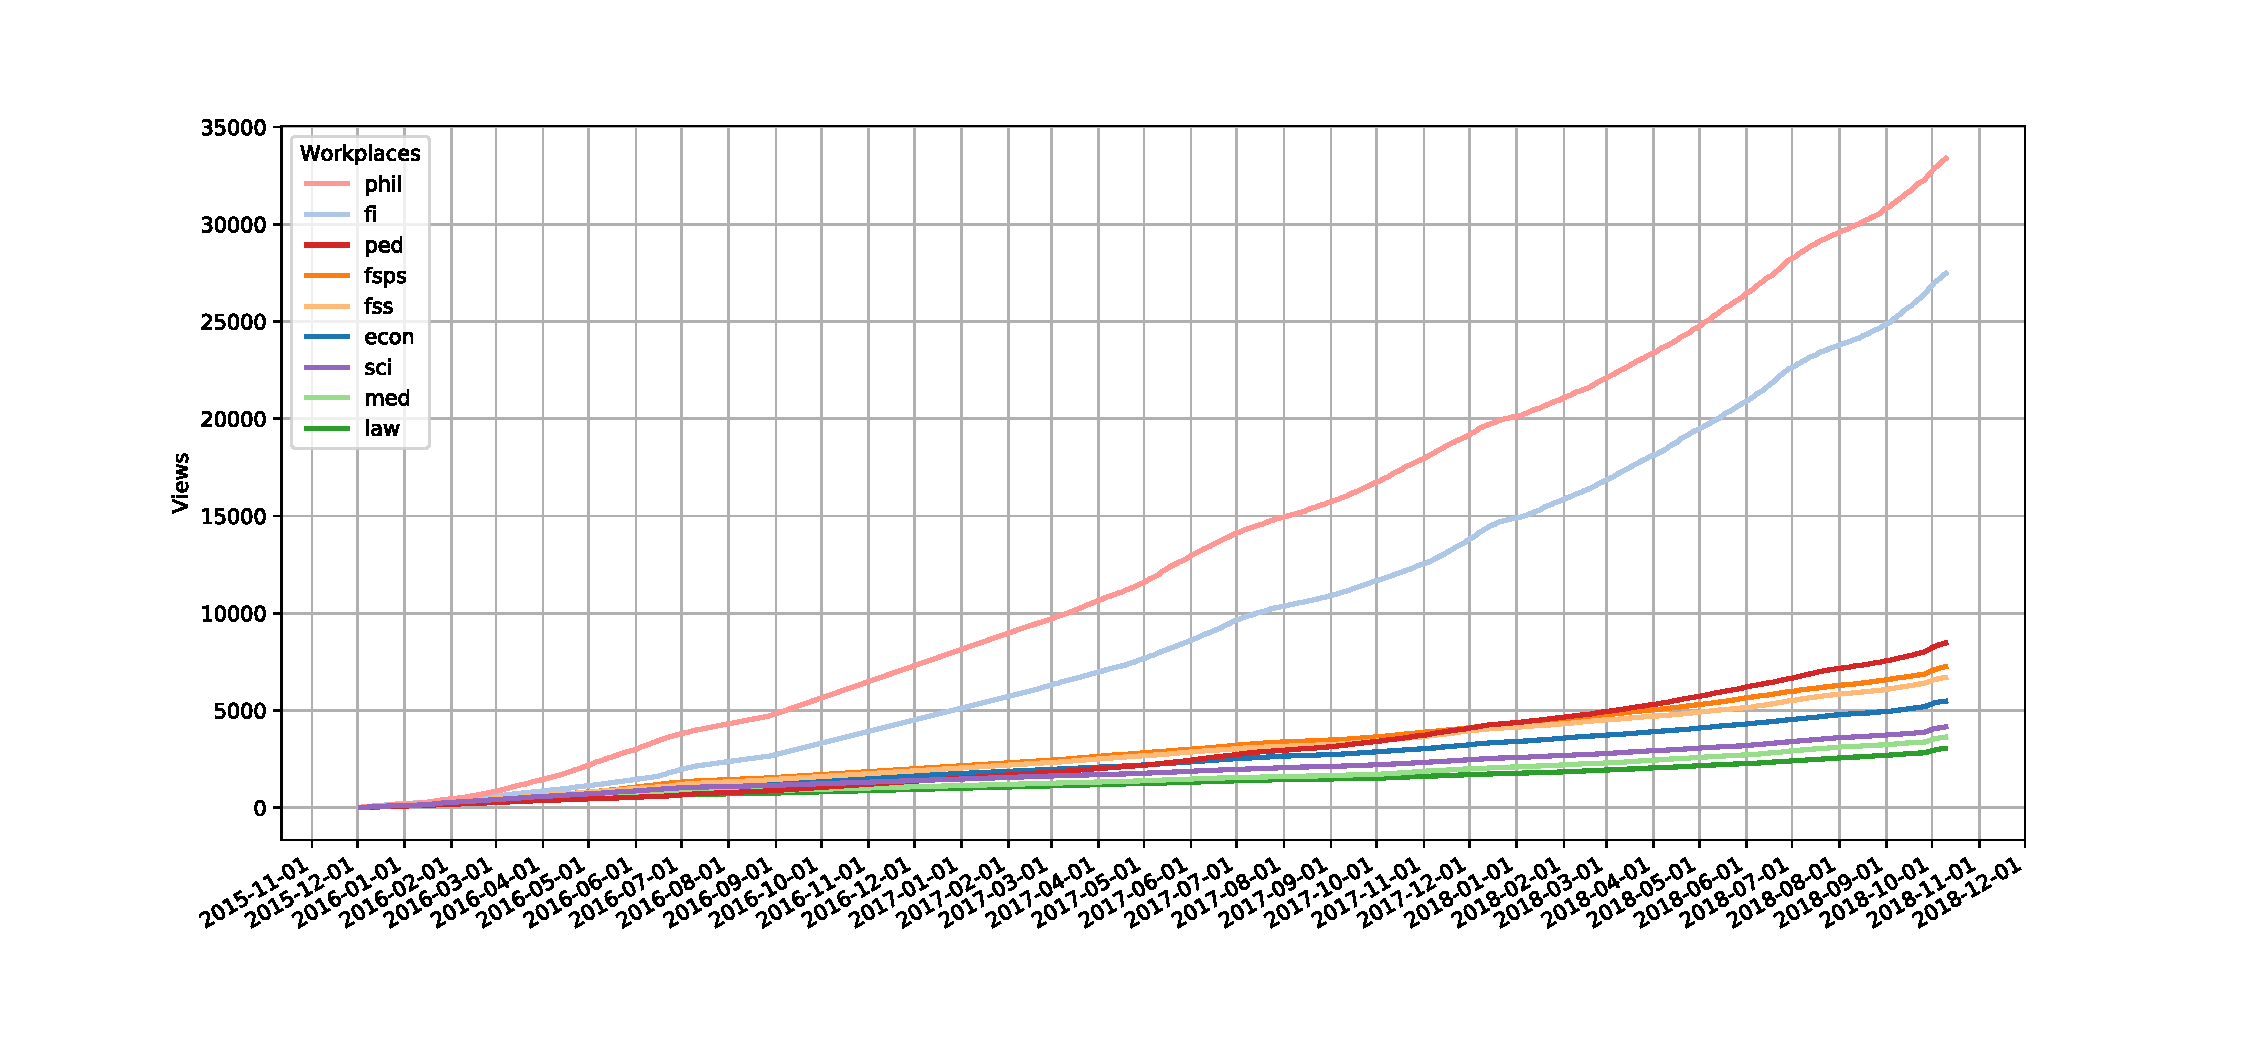
\includegraphics[width=1.1\textwidth]{figs/fibeamer}
\end{frame}

\begin{frame}{Počty přístupů k~šabloně mubeamer podle pracovišť}
\kern-1.5em\leavevmode\relax
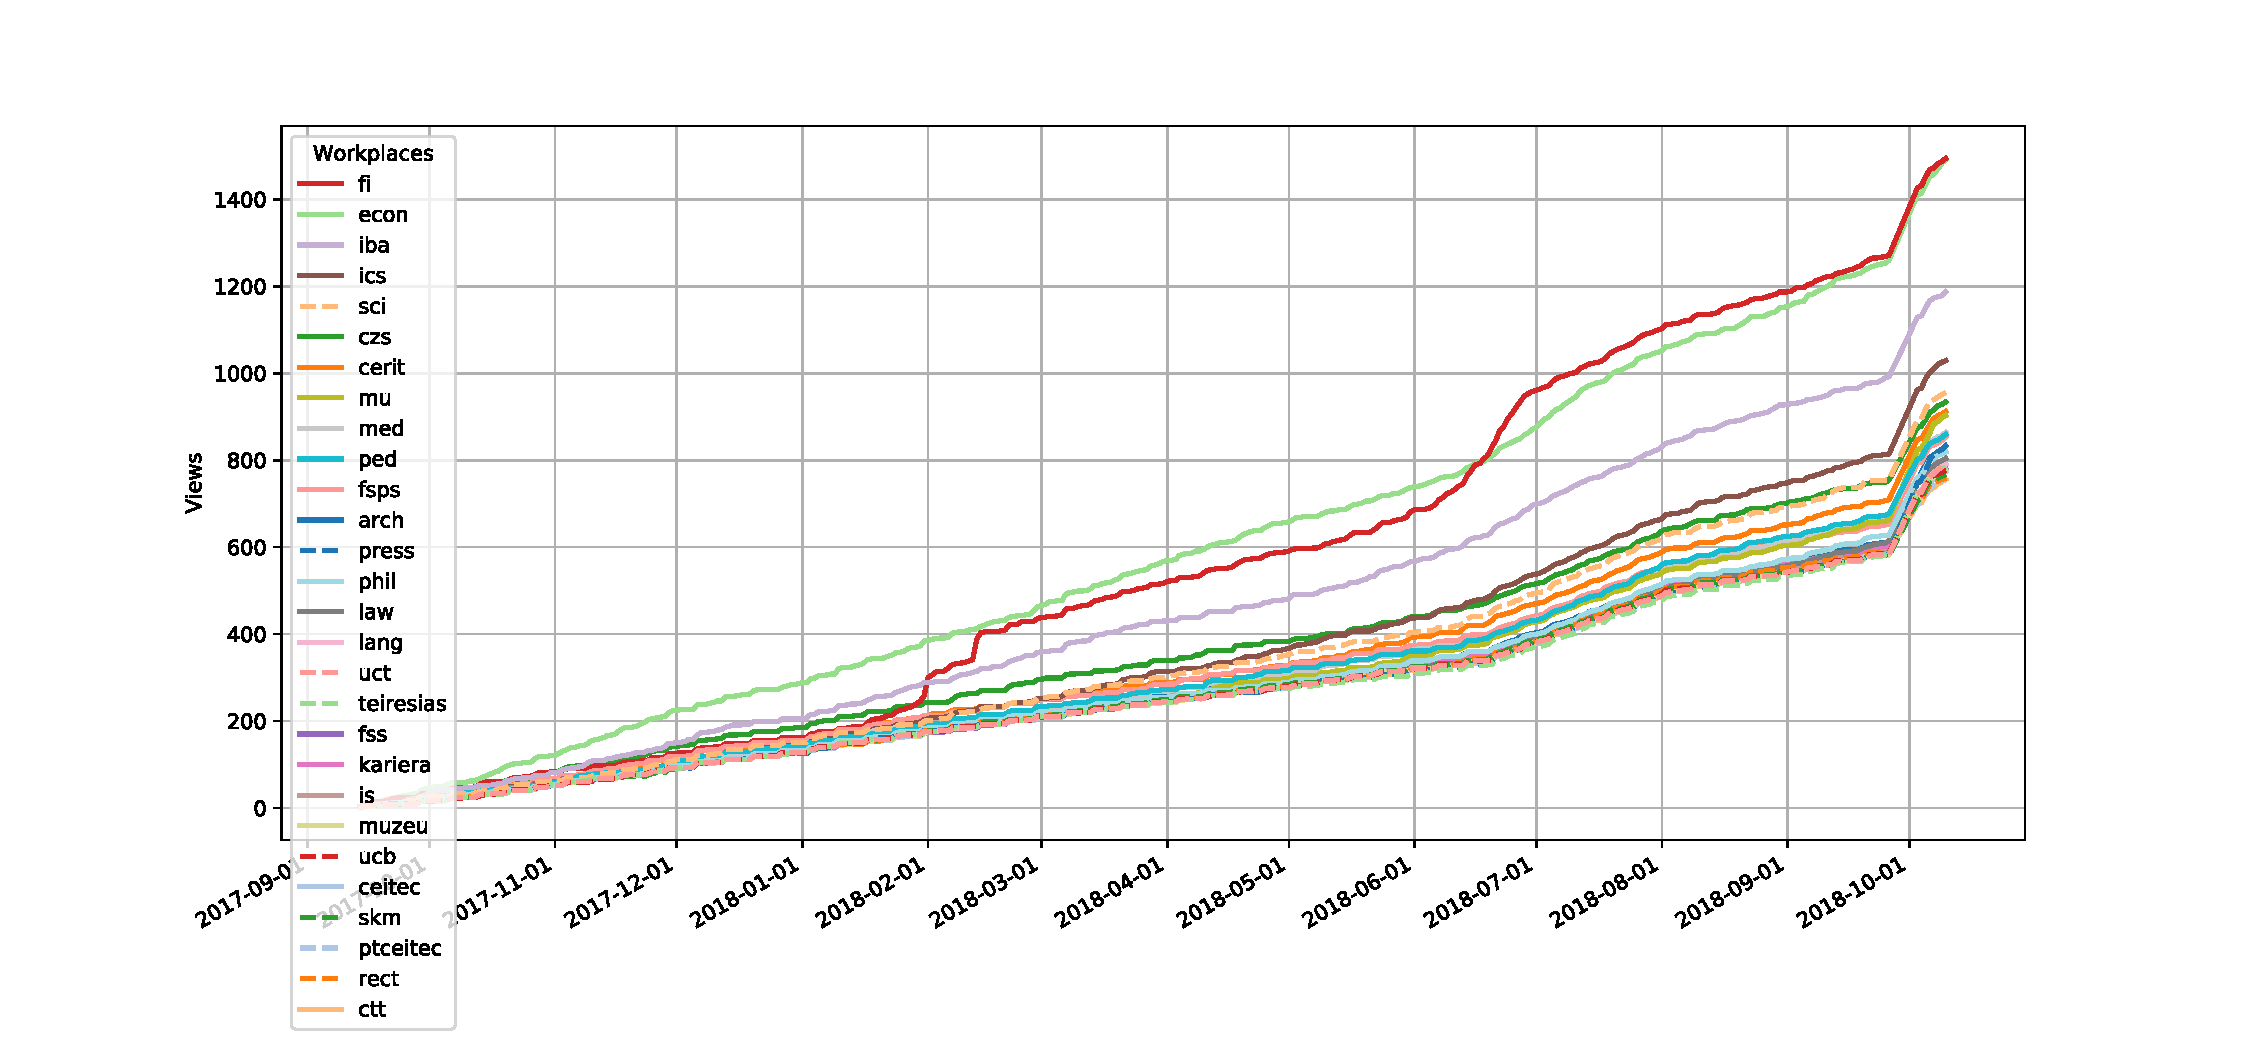
\includegraphics[width=\textwidth]{figs/mubeamer}
\end{frame}

\subsection{Šablona muletter}

\begin{frame}{Šablona muletter}
\begin{itemize}
\item V~roce 2017 vznikla na FI \alert{šablona muletter pro sazbu dopisů podle JVS MU 2016 na 28 pracovištích MU}.
\end{itemize}

\begin{block}{Příklad}
Pracoviště odesílatele lze snadno změnit bez zásahu do samotného obsahu dokumentu. Zároveň lze snadno sázet stovky dopisů na základě tabulkových dat z~Microsoft Office a~strojově generovat jejich obsah.
\end{block}
\end{frame}

\begin{frame}{Počty přístupů k~šabloně muletter podle pracovišť}
\kern-1.5em\leavevmode\relax
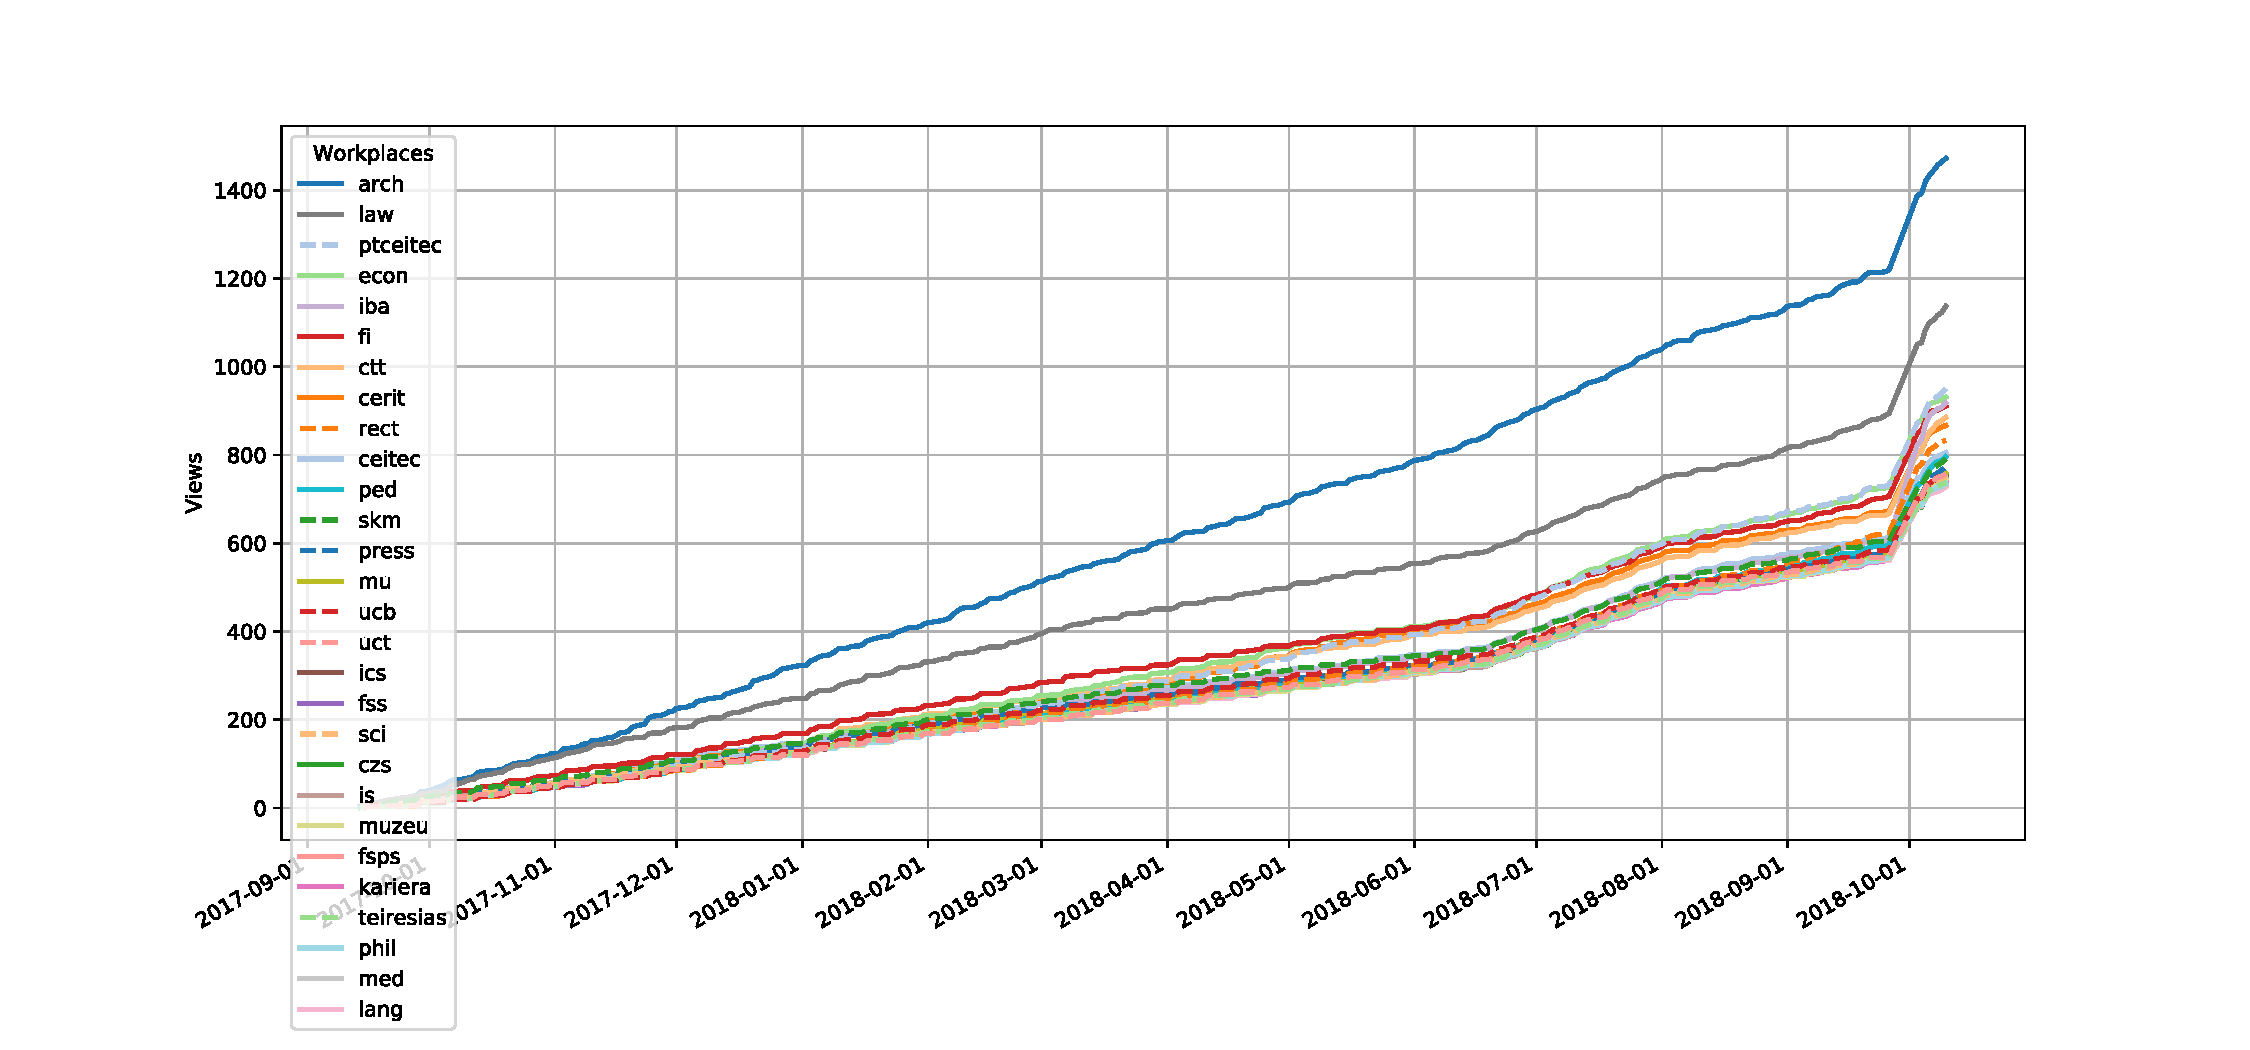
\includegraphics[width=\textwidth]{figs/muletter}
\end{frame}

\section{Závěr}

\begin{frame}{Závěr}
\begin{itemize}
\item \alert{\TeX{} má na MU čtvrt století dlouhou tradici} a~významně se podílí na produkci kvalitních výstupů, jak provozních, tak výzkumných.
\item Investice do \TeX u je investicí do \alert{kvalitní sazby} a~\alert{snadné automatizovatelnosti}, jeho užití v~rámci databázových výstupů ISu se již mnohokráte zúročila. 
\item Financování vývoje a provozu \TeX ové podpory šla doposud v~drtivé většině k~tíži FI MU přesto, že je \alert{široce užívaná napříč celou univerzitou} (přímo v~\odkaz{https://www.overleaf.com/edu/fimuni}{Overleaf.com}, nebo nepřímo v~IS MU), jak ukazují statistiky užití.
\item Současné šablony splňují pouze JVS MU 2016, ne JVS MU 2018.
\end{itemize}
\end{frame}

\section{Bibliografie}

\begin{frame}{Bibliografie}
\bibliography{main}
\end{frame}

\begin{frame}[plain]
\vfill
\centerline{Děkuji za pozornost!}
\vfill\vfill
\end{frame}

\end{document}